\chapter{Pohon Filogeni dan Jam Molekul}\label{ch:b2:phylogenetic-trees}

Pada tahun 1965 dua ahli kimia, Emile Zuckerkandl dan Linus Pauling,
membandingkan runtunan asam amino hemoglobin dari segelintir vertebrata
lalu memperhatikan sesuatu yang tidak akan dapat dilihat seorang ahli
anatomi: jumlah perbedaan antara dua spesies sebanding dengan waktu
sejak moyangnya berpisah, sebagaimana dibaca dari fosilnya. Sebuah
molekul menyimpan waktu. Dalam satu dasawarsa Carl Woese telah memakai
satu gen, yaitu RNA subunit ribosom yang kecil, untuk menggambar pohon
seluruh kehidupan dan untuk menemukan di dalamnya sebuah domain ketiga,
yaitu arkea, yang tidak dapat dibedakan mikroskop mana pun dari
bakteri. Bab ini membahas penyusunan ulang sejarah dari kemiripannya:
apa arti sebuah pohon, bagaimana sebuah pohon dibangun dari sifat dan
dari jaraknya, bagaimana runtunan dibuat menyatakan waktu, dan jebakan
--- pemusatan, laju yang tak sama, kejenuhan, cabang yang panjang ---
yang harus diketahui seorang pembaca pohon.

\section{Membaca sebuah pohon}

\begin{definition}[Filogeni, klad, homologi]\label{def:b2:phylogenetic-trees:tree}
\index{filogeni}\index{klad}\index{kelompok monofiletik}\index{kelompok parafiletik}%
\index{kelompok polifiletik}\index{homologi}\index{analogi}\index{sinapomorfi}
Sebuah \emph{filogeni} adalah sebuah pohon yang ujungnya adalah spesies
(atau gen, atau individu) yang dibandingkan, yang simpul dalamnya
adalah moyang bersamanya, dan yang akarnya adalah moyang tertua
semuanya. Urutan percabangannya sajalah yang membawa sejarahnya:
simpulnya boleh diputar dengan bebas, dan hanya persarangannya yang
berarti. Sebuah \emph{klad} atau \emph{kelompok monofiletik} adalah
seorang moyang beserta \emph{seluruh} keturunannya (burung; mamalia;
burung dan buaya bersama-sama); sebuah kelompok \emph{parafiletik}
adalah seorang moyang dengan sebagian keturunannya ditinggalkan
(``reptil'' tanpa burung, ``ikan'' tanpa tetrapoda, ``prokariota'');
sebuah kelompok \emph{polifiletik} menyatukan keturunan moyang yang
berbeda lewat sebuah kemiripan yang dievolusikannya secara terpisah
(``hewan berdarah panas''). Sebuah sifat yang dibagi dua spesies karena
moyangnya memilikinya adalah sebuah \emph{homologi} (tulang sayap
kelelawar dan sirip paus); sifat yang dievolusikannya secara bebas
adalah sebuah \emph{analogi} atau \emph{homoplasi} (sayap kelelawar dan
sayap burung sebagai sayap, mata kamera vertebrata dan gurita). Hanya
homologi yang mencatat sejarah, dan di antaranya hanya keadaan
\emph{turunan} yang dibagi sebuah kelompok --- yaitu
\emph{sinapomorfinya}, kata Hennig --- yang membatasi sebuah klad: bulu
membatasi burung, sedangkan keadaan moyang ``tanpa bulu'' tidak
membatasi apa pun.
\end{definition}

\begin{omfigure}
\begin{tikzpicture}[every node/.style={font=\scriptsize}, >=stealth, line width=0.8pt]
  \coordinate (root) at (0,0);
  \coordinate (n1) at (1.2,0.9); \coordinate (n2) at (2.4,1.6); \coordinate (n3) at (3.6,2.3);
  \draw (root) -- (1.4,-1.3) node[right] {mamalia};
  \draw (root) -- (n1);
  \draw (n1) -- (4.8,-0.1) node[right] {kura-kura};
  \draw (n1) -- (n2);
  \draw (n2) -- (4.8,0.9) node[right] {kadal, ular};
  \draw (n2) -- (n3);
  \draw (n3) -- (4.8,1.9) node[right] {buaya};
  \draw (n3) -- (4.8,3.0) node[right] {burung};
  \fill (root) circle (1.6pt); \fill (n1) circle (1.6pt); \fill (n2) circle (1.6pt); \fill (n3) circle (1.6pt);
  \node[left] at (root) {amniota};
  % groups
  \draw[omThm, thick, rounded corners=6pt] (3.1,1.55) rectangle (6.9,3.4);
  \node[omThm, anchor=south west] at (3.1,3.4) {arkosaur: monofiletik};
  \draw[omExo!80!black, thick, dashed, rounded corners=6pt] (2.2,-0.5) -- (2.2,2.2) -- (7.1,2.2) -- (7.1,-0.5) -- cycle;
  \node[omExo!80!black, anchor=north east] at (7.1,-0.55) {``reptil'' tanpa burung: parafiletik};
  \node[anchor=west, align=left, text width=4.2cm] at (7.9,1.3) {sinapomorfi:\\ $\bullet$ telur amnion (semuanya)\\ $\bullet$ lubang antorbital pada tengkoraknya (arkosaur)\\ $\bullet$ bulu (burung)};
\end{tikzpicture}

{\small Membaca sebuah pohon. Burung bersarang di dalam reptilnya:
buaya lebih dekat kepada burung daripada kepada kadal. Kelompok bernama
``reptil'' adalah seorang moyang dengan satu garis keturunan
disingkirkan --- sebuah jenjang parafiletik, bukan sebuah \omterm{def:b2:phylogenetic-trees:tree}{klad}.}
\end{omfigure}

\begin{omfigure}
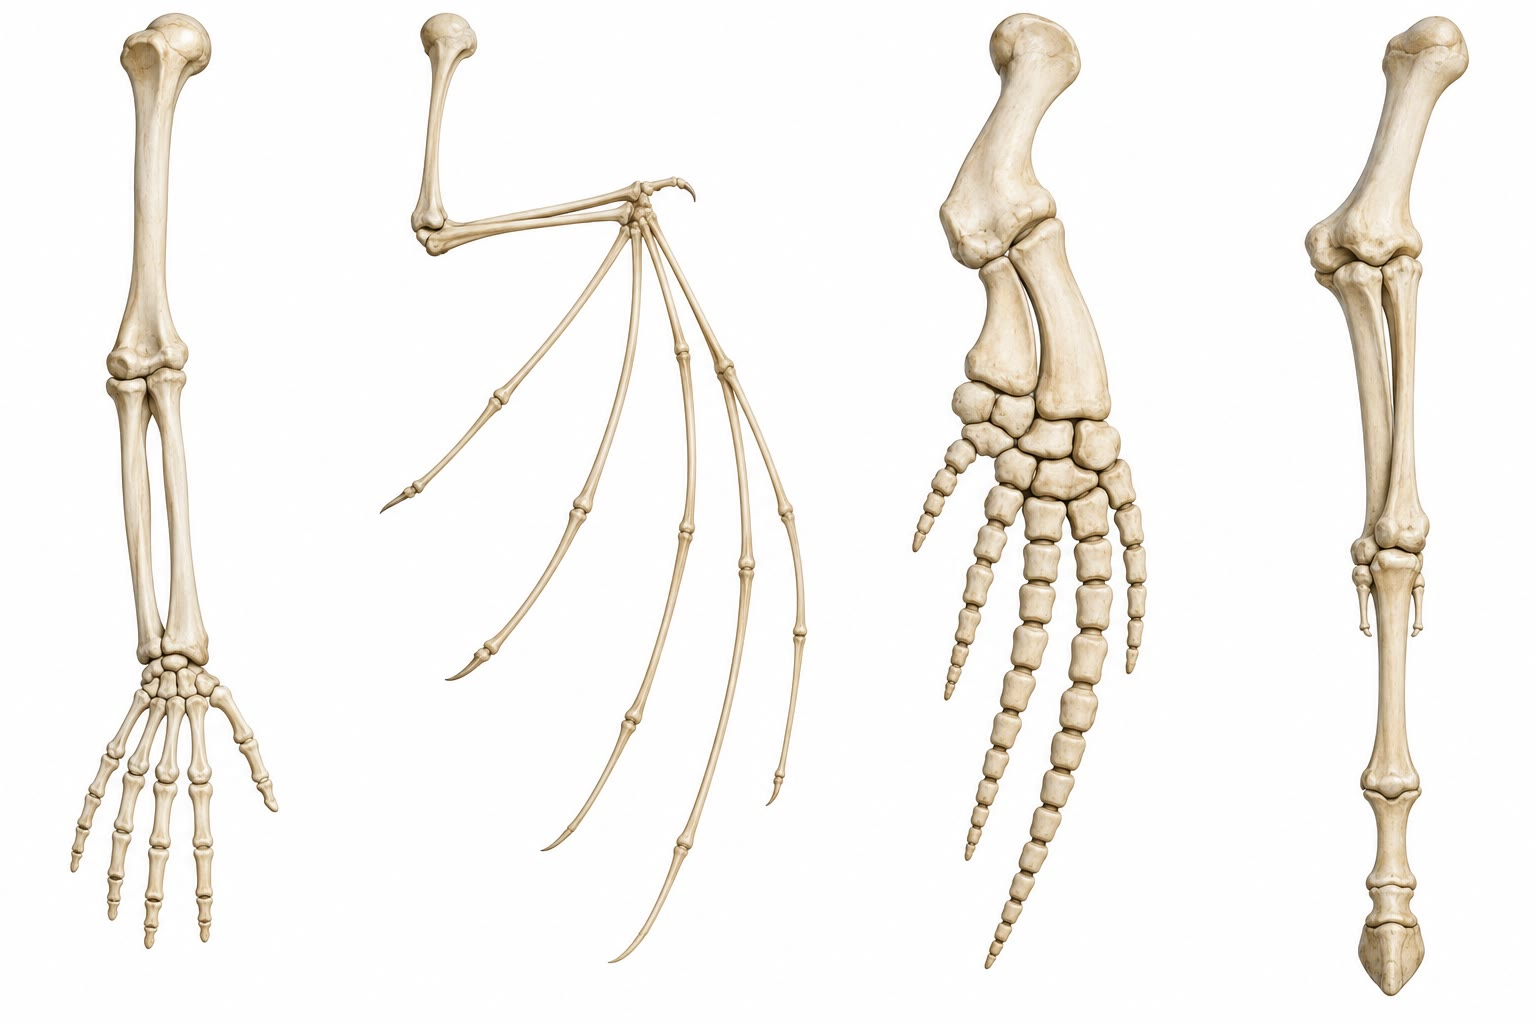
\includegraphics[width=0.44\linewidth]{images/book4/ai/b4-24-homologous-forelimbs.jpg}\hspace{0.04\linewidth}
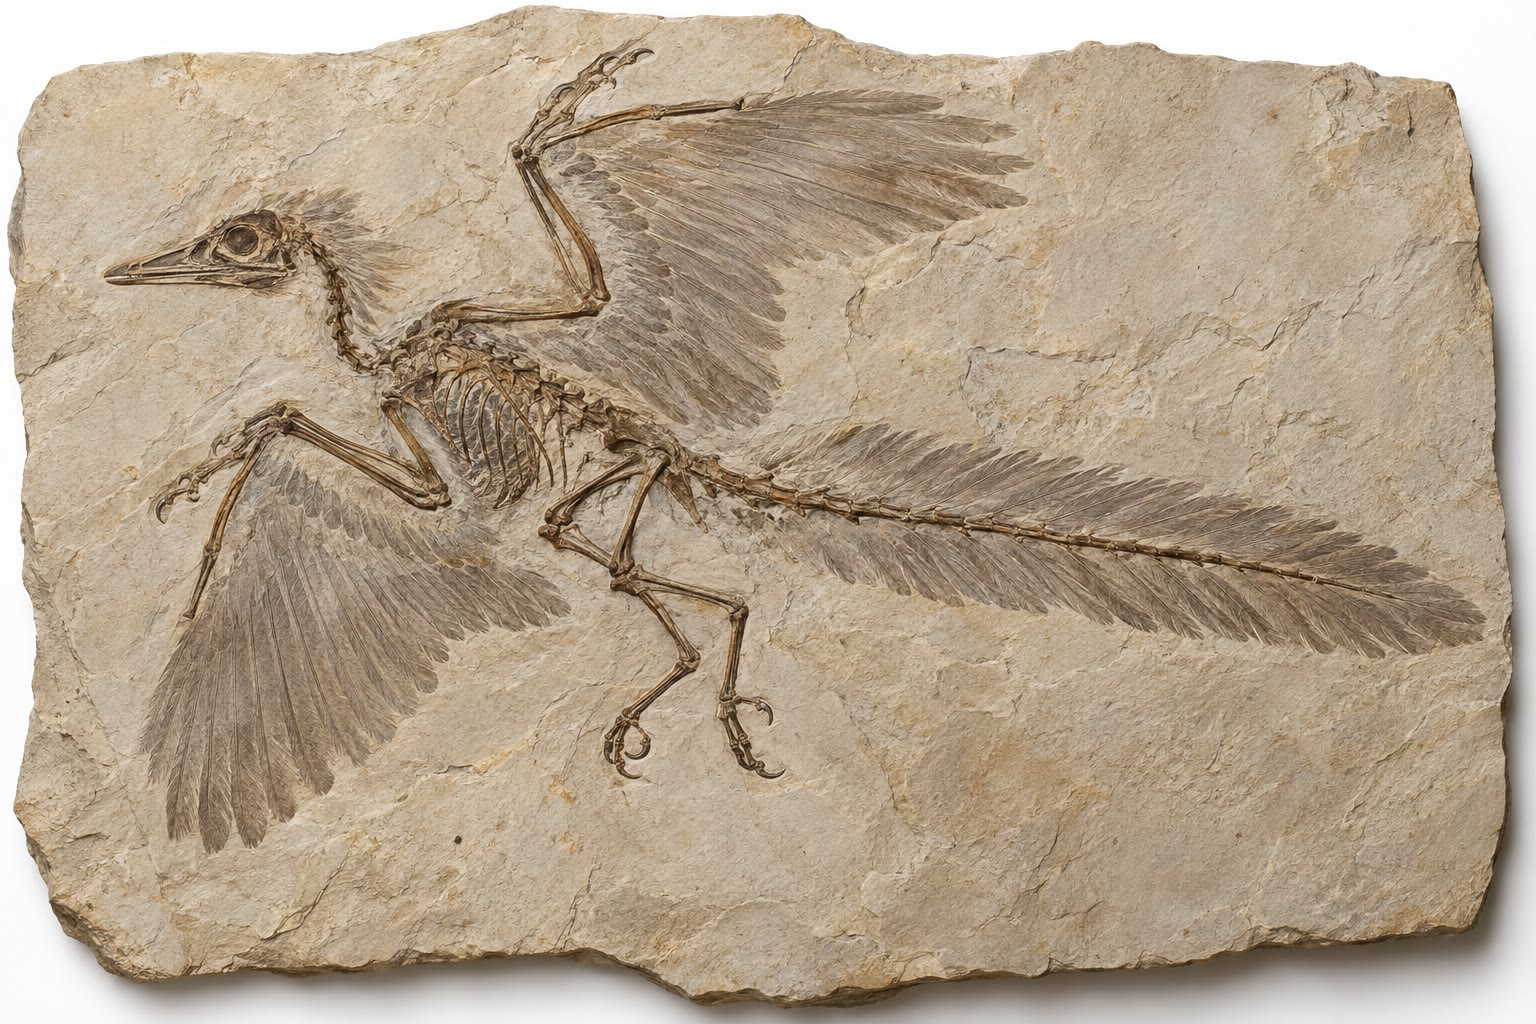
\includegraphics[width=0.44\linewidth]{images/book4/ai/b4-24-archaeopteryx.jpg}

{\small \omterm{def:b2:phylogenetic-trees:tree}{Homologi} dan catatannya. Kiri: tulang yang sama --- humerus,
radius dan ulna, pergelangan, lima jari --- pada sebuah lengan, sebuah
sayap, sebuah sirip, dan sebuah kaki. Kanan: \emph{Archaeopteryx},
dengan gigi, jari bercakar, dan ekor bertulang panjang seekor dinosaurus
kecil serta bulu seekor burung.}
\end{omfigure}

\section{Membangun pohon dari sifatnya}

\begin{method}[Parsimoni]\label{meth:b2:phylogenetic-trees:parsimony}
\index{parsimoni}\index{kelompok luar}\index{bootstrap}
Nilailah sifatnya (keadaan morfologis atau kedudukan runtunan yang
dijajarkan) bagi tiap taksonnya. Bagi tiap pohon yang mungkin, cacahlah
jumlah minimum perubahan sifat yang diperlukan untuk menerangkan
datanya pada pohon itu; pohon yang paling parsimonis memerlukan paling
sedikit. Akarkan pohonnya dengan sebuah \emph{\omterm{meth:b2:phylogenetic-trees:parsimony}{kelompok luar}}, yaitu
sebuah takson yang diketahui terletak di luar kelompok yang dipelajari.
Karena jumlah pohon tak berakar bagi $n$ takson adalah $1\cdot 3\cdot
5\cdots(2n - 5)$ --- tiga bagi empat takson, $2\times 10^{6}$ bagi
sepuluh, $10^{20}$ bagi dua puluh --- pencariannya menyeluruh hanya bagi
himpunan yang kecil dan bersifat heuristik di luar itu. Keyakinannya
diukur dengan \emph{bootstrap}: contohlah ulang sifatnya dengan
pengembalian seribu kali, bangun ulang pohonnya tiap kalinya, lalu
catat seberapa sering tiap \omterm{def:b2:phylogenetic-trees:tree}{kladnya} muncul lagi; sebuah \omterm{def:b2:phylogenetic-trees:tree}{klad} yang
ditemukan pada \qty{95}{\%} contoh ulangnya tersokong dengan baik,
sedangkan yang ditemukan pada separuhnya tidak.
\end{method}

\begin{example}[Empat takson, lima tapak]\label{ex:b2:phylogenetic-trees:parsimony}
Runtunan $A = \mathrm{AAGCT}$, $B = \mathrm{AAGCC}$, $C =
\mathrm{GGACT}$, $D = \mathrm{GGATC}$. Pada pohon $((A,B),(C,D))$,
tapak 1, 2, dan 3 masing-masing berubah sekali (pada cabang dalamnya),
tapak 4 sekali ($\mathrm{C}\to\mathrm{T}$ pada $D$) dan tapak 5 dua kali
($\mathrm{T}\to\mathrm{C}$ pada $B$ dan pada $D$): enam langkah. Pada
$((A,C),(B,D))$, tapak 1--3 masing-masing memerlukan dua perubahan,
tapak 4 dan 5 masing-masing satu: delapan. Pada $((A,D),(B,C))$:
sembilan. Pohon yang pertama paling parsimonis, dengan selisih dua
langkah; ketiga tapak yang menyokongnya adalah \omterm{def:b2:phylogenetic-trees:tree}{sinapomorfinya}, dan
tapak 5 adalah sebuah homoplasi padanya --- perubahan yang sama yang
terjadi dua kali, sebuah kenyataan hidup pada tiap himpunan data yang
nyata.
\end{example}

\begin{omfigure}
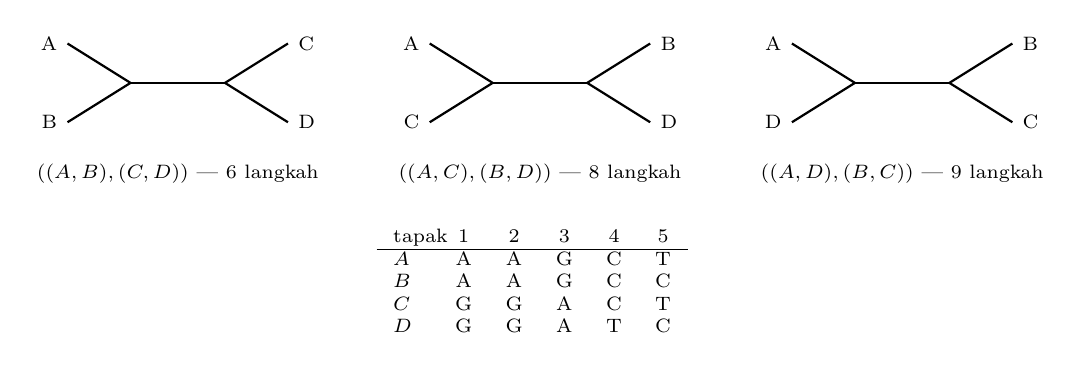
\begin{tikzpicture}[every node/.style={font=\scriptsize}, line width=0.8pt]
  \foreach \x/\a/\b/\c/\d/\steps/\lab in {0/A/B/C/D/6/{$((A,B),(C,D))$ --- 6 langkah}, 4.6/A/C/B/D/8/{$((A,C),(B,D))$ --- 8 langkah}, 9.2/A/D/B/C/9/{$((A,D),(B,C))$ --- 9 langkah}} {
    \begin{scope}[xshift=\x cm]
      \draw (0,1.6) node[left] {\a} -- (0.8,1.1) -- (0,0.6) node[left] {\b};
      \draw (0.8,1.1) -- (2.0,1.1);
      \draw (2.8,1.6) node[right] {\c} -- (2.0,1.1) -- (2.8,0.6) node[right] {\d};
      \node[anchor=north] at (1.4,0.2) {\lab};
    \end{scope}
  }
  \node[anchor=north] at (5.9,-0.6) {\begin{tabular}{l@{\ }ccccc} tapak & 1 & 2 & 3 & 4 & 5 \\ \hline $A$ & A & A & G & C & T \\ $B$ & A & A & G & C & C \\ $C$ & G & G & A & C & T \\ $D$ & G & G & A & T & C \end{tabular}};
\end{tikzpicture}

{\small Ketiga pohon tak berakar bagi empat takson, yang dinilai
terhadap penjajaran lima tapak di bawahnya. Tapak 1--3 berubah sekali
pada pohon yang pertama dan dua kali pada pohon lainnya; tapak 4
berubah pada satu takson saja dan tidak dapat memutuskan, sedangkan
tapak 5 mengelompokkan $A$ dengan $C$ sehingga menyukai pohon yang
ketiga terhadap keduanya.}
\end{omfigure}

\section{Membangun pohon dari jaraknya}

\begin{method}[Menggugus menurut jarak: UPGMA]\label{meth:b2:phylogenetic-trees:upgma}
\index{UPGMA}\index{penggabungan tetangga}\index{matriks jarak}
Dari jarak berpasangan antara $n$ takson (perbedaan tiap tapak, yang
dikoreksi seperti di bawah), gabungkan pasangan yang terdekat menjadi
sebuah gugus yang ditaruh pada sebuah simpul setinggi separuh jaraknya;
gantikan pasangannya dengan gugusnya, yang jaraknya ke tiap takson
lainnya adalah rerata jarak anggotanya; ulangi sampai satu gugus
tersisa. Hasilnya adalah sebuah pohon berakar yang seluruh ujungnya
berada pada tinggi yang sama --- ia menganggap sebuah laju perubahan
yang tetap pada tiap cabangnya, yaitu sebuah \omterm{thm:b2:phylogenetic-trees:clock}{jam molekul}. Ketika lajunya
berbeda antargaris keturunan, metodenya mengelompokkan garis keturunan
yang cepat berevolusi bersama-sama apa pun sejarahnya;
\emph{\omterm{meth:b2:phylogenetic-trees:upgma}{penggabungan tetangga}}, yang pada tiap langkahnya menggabungkan
pasangan yang penyatuannya paling memendekkan seluruh pohonnya, tidak
menganggap sebuah jam dan merupakan metode cepat yang baku bagi
himpunan data yang besar.
\end{method}

\begin{example}[UPGMA]\label{ex:b2:phylogenetic-trees:upgma}
Jaraknya (dalam perbedaan tiap seratus tapak): $AB = 4$, $AC = 8$,
$AD = 10$, $BC = 8$, $BD = 10$, $CD = 6$. Gabungkan $A$ dan $B$ pada
tinggi 2; lalu $d(AB, C) = 8$, $d(AB, D) = 10$, $d(C,D) = 6$: gabungkan
$C$ dan $D$ pada tinggi 3; akhirnya
$d(AB, CD) = (8 + 10 + 8 + 10)/4 = 9$: gabungkan kedua gugusnya pada tinggi $4.5$. Pohonnya adalah
$((A,B),(C,D))$, dan jika lajunya $10^{-9}$ penggantian tiap tapak tiap
tahun akarnya berumur $0.045/10^{-9} = 45$ juta tahun.
\end{example}

\begin{omfigure}
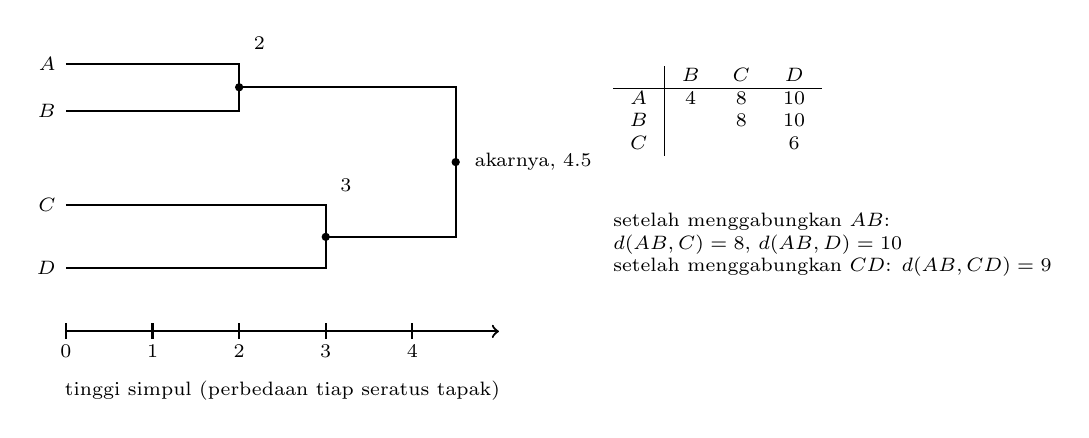
\begin{tikzpicture}[every node/.style={font=\scriptsize}, line width=0.8pt, x=1.1cm]
  \draw[->] (0,-0.4) -- (5,-0.4); \foreach \h in {0,1,2,3,4} \draw (\h,-0.5) -- (\h,-0.3) node[below=4pt] {\h};
  \node[anchor=north] at (2.5,-0.9) {tinggi simpul (perbedaan tiap seratus tapak)};
  % A,B join at 2, C,D at 3, root at 4.5 ; draw as rooted tree, root on the right
  \draw (0,3.0) node[left] {$A$} -- (2,3.0) -- (2,2.4) -- (0,2.4) node[left] {$B$};
  \draw (0,1.2) node[left] {$C$} -- (3,1.2) -- (3,0.4) -- (0,0.4) node[left] {$D$};
  \draw (2,2.7) -- (4.5,2.7) -- (4.5,0.8) -- (3,0.8);
  \fill (2,2.7) circle (1.5pt); \fill (3,0.8) circle (1.5pt); \fill (4.5,1.75) circle (1.5pt);
  \node[anchor=west] at (4.6,1.75) {akarnya, 4.5};
  \node[anchor=south west] at (2.05,3.05) {2};
  \node[anchor=south west] at (3.05,1.25) {3};
  \node[anchor=west, align=left] at (6.2,2.4) {\begin{tabular}{c|ccc} & $B$ & $C$ & $D$ \\ \hline $A$ & 4 & 8 & 10 \\ $B$ & & 8 & 10 \\ $C$ & & & 6 \end{tabular}};
  \node[anchor=west, align=left] at (6.2,0.7) {setelah menggabungkan $AB$:\\ $d(AB,C) = 8$, $d(AB,D) = 10$\\ setelah menggabungkan $CD$: $d(AB,CD) = 9$};
\end{tikzpicture}

{\small UPGMA pada empat takson. Tiap simpulnya duduk pada separuh
jarak antara gugus yang ia gabungkan; tiap ujungnya berakhir pada
tinggi nol, sebagaimana yang dituntut sebuah jam.}
\end{omfigure}

\section{Jam molekulnya}

\begin{theorem}[Penggantian sebagai proses Poisson, dan koreksi bagi kena berulang]\label{thm:b2:phylogenetic-trees:clock}
\index{jam molekul}\index{koreksi Jukes--Cantor}\index{kejenuhan}
Jika penggantian pada sebuah tapak terjadi pada laju tetap $k$ tiap
tahun, secara bebas antartapak, jumlah yang menimbun sepanjang sebuah
garis keturunan dalam waktu $t$ berdistribusi Poisson dengan rerata
$kt$, dan jumlah harapan yang memisahkan dua garis keturunan yang
memencar $t$ tahun yang lalu adalah
\[
d = 2kt
\]
penggantian tiap tapak --- yaitu \emph{\omterm{thm:b2:phylogenetic-trees:clock}{jam molekulnya}}. Bagian $p$
tapak yang berbeda yang teramati lebih kecil daripada $d$, karena
sebuah tapak yang terkena dua kali boleh jadi kembali ke basa aslinya
atau cocok secara kebetulan; dengan empat basa yang berubah pada laju
yang sama,
\[
p = \tfrac{3}{4}\bigl(1 - e^{-4d/3}\bigr), \qquad
d = -\tfrac{3}{4}\ln\bigl(1 - \tfrac{4}{3}p\bigr),
\]
yaitu koreksi \emph{Jukes--Cantor}. Ketika $d$ bertambah, $p$ menjenuh
pada $3/4$ --- dua runtunan acak bersesuaian pada seperempat tapaknya
--- dan di luar $p \approx 0.5$ koreksinya membesarkan tiap galat
pencontohannya: sebuah gen yang telah berubah sebanyak itu telah
berhenti menyimpan waktu. Gen yang lambat (RNA ribosom, histon)
menanggali cabang yang dalam, sedangkan yang cepat (DNA mitokondria,
intron) menanggali yang baru.
\end{theorem}
\begin{proof}
Misalkan $q(t)$ adalah peluang bahwa sebuah tapak masih membawa basa
aslinya setelah waktu $t$. Ia hilang pada laju $k$ dan diperoleh
kembali, dari salah satu dari tiga basa lainnya, pada laju $k/3$:
$\mathrm{d}q/\mathrm{d}t = -kq + \tfrac{k}{3}(1 - q) = \tfrac{k}{3} -
\tfrac{4k}{3}q$, yang penyelesaiannya dengan $q(0) = 1$ adalah $q = \tfrac14 +
\tfrac34 e^{-4kt/3}$. Dua garis keturunan yang dipisahkan waktu total
$2t$ --- menurut kesetangkupannya, sama dengan satu garis keturunan
yang berevolusi selama $2t$ --- bersesuaian pada sebuah tapak dengan
peluang $\tfrac14 + \tfrac34 e^{-4d/3}$ dengan $d =
2kt$, sehingga $p = 1 - q = \tfrac34(1 - e^{-4d/3})$; membalikkannya memberikan koreksinya.
Cacahan Poissonnya menyusul dari peristiwa yang tetap dan bebas,
seperti pada fisika peluruhan radioaktif, dan simpangan bakunya
$\sqrt{kt}$ menetapkan ketelitian tanggal mana pun: sebuah gen berisi
$L$ tapak dengan $dL$ penggantian yang teramati menanggali sebuah
pemencaran sampai ketelitian nisbi kira-kira $1/\sqrt{dL}$.
\end{proof}
\begin{proof}[Bukti eksperimental]
Zuckerkandl dan Pauling (1965) menemukan perbedaan antara hemoglobin
kuda, manusia, sapi, dan lainnya sebanding dengan umur fosil
pembelahannya, lalu mengusulkan jamnya. Fitch dan Margoliash (1967)
membangun sebuah pohon berisi dua puluh spesies dari sitokrom $c$ saja
lalu memperoleh kembali, dari satu protein tunggal, pengelompokan
klasik vertebrata, serangga, dan jamur. Uji metode yang menentukan
adalah \omterm{def:b2:phylogenetic-trees:tree}{filogeni} eksperimental Hillis dan rekannya (1992): mereka
membiakkan bakteriofag T7 lewat sebuah rangkaian bercabang berisi
delapan garis keturunan yang diketahui di bawah sebuah mutagen,
meruntunkan hasilnya, lalu memberikan runtunannya kepada metode
pembangun pohon secara buta --- metode parsimoni, jarak, dan
kebolehjadian semuanya memperoleh kembali pohon yang benar, dan
parsimoninya menyusun ulang runtunan moyangnya dengan ketepatan di
atas \qty{98}{\%}.
\end{proof}

\begin{omfigure}
\begin{tikzpicture}
\begin{axis}[
  width=0.7\linewidth, height=5.4cm,
  axis x line=bottom, axis y line=left,
  xmin=0, xmax=2.5, ymin=0, ymax=1.05,
  xlabel={penggantian sebenarnya tiap tapak, $d$}, ylabel={perbedaan teramati, $p$},
  xlabel style={font=\small, at={(axis description cs:0.5,-0.13)}, anchor=north},
  ylabel style={font=\small},
  tick label style={font=\small}, ytick={0,0.25,0.5,0.75,1},
  legend style={font=\scriptsize, at={(0.97,0.35)}, anchor=east, draw=none},
  clip=false,
]
\addplot[very thick, omDef, domain=0:2.5, samples=80] {0.75*(1-exp(-4*x/3))};
\addlegendentry{$p = \tfrac34(1 - e^{-4d/3})$}
\addplot[thick, gray, dashed, domain=0:1.05, samples=2] {x};
\addlegendentry{$p = d$: tanpa kena berulang}
\draw[dotted, gray] (axis cs:0,0.75) -- (axis cs:2.5,0.75); \node[font=\scriptsize, anchor=south east] at (axis cs:2.5,0.75) {kejenuhan, $p = 3/4$};
\draw[<->, omThm, thick] (axis cs:0.383,0.30) -- (axis cs:0.383,0.383); \node[font=\scriptsize, omThm, anchor=west] at (axis cs:0.5,0.22) {$p = 0.30$ berarti $d = 0.38$};
\end{axis}
\end{tikzpicture}

{\small Kena berulang. Bagian tapak yang berbeda yang teramati naik
bersama jumlah penggantian yang sebenarnya lalu menjenuh; sebuah $p$
yang mentah menaksir terlalu rendah tiap jaraknya dan memampatkan
cabang dalam sebuah pohon.}
\end{omfigure}

\begin{proposition}[Jebakan jamnya dan jebakan pohonnya]\label{prop:b2:phylogenetic-trees:pitfalls}
\index{tarikan cabang panjang}\index{keheterogenan laju}%
\index{penyortiran garis keturunan tak lengkap}\index{kebolehjadian (filogenetika)}
Jamnya hanya tetap secara hampiran: lajunya berbeda antargen sampai
seratus kali lipat (menurut fungsinya --- histon H4 telah mengubah dua
residu dalam satu miliar tahun, sedangkan fibrinopeptida berubah tiap
beberapa juta tahun), antartapak di dalam sebuah gen (kedudukan kodon
ketiga, intron, dan simpul berubah paling cepat), dan antargaris
keturunan (hewan pengerat berdetak lebih cepat daripada primata, dengan
generasinya yang lebih pendek dan laju metabolismenya yang lebih
tinggi). Karena itu tiap jamnya memerlukan \emph{kalibrasi} oleh sebuah
fosil atau sebuah peristiwa geologis bertanggal, dan tanggalnya membawa
galat Poisson di atas beserta galat kalibrasinya sendiri. Pohonnya
memiliki jebakannya sendiri. \emph{\omterm{prop:b2:phylogenetic-trees:pitfalls}{Tarikan cabang panjang}}: dua garis
keturunan yang masing-masing telah banyak berubah berbagi banyak tapak
secara kebetulan, dan parsimoninya menggabungkan keduanya apa pun
sejarahnya --- obatnya adalah pencontohan yang lebih rapat untuk
mematahkan cabangnya dan sebuah metode yang memodelkan lajunya.
\emph{Pemusatan} menghasilkan \omterm{def:b2:phylogenetic-trees:tree}{sinapomorfi} palsu. \emph{Penyortiran
garis keturunan yang tak lengkap}: pohon sebuah gen tidak harus menjadi
pohon spesiesnya ketika spesiasinya saling menyusul dengan cepat,
karena polimorfisme moyangnya menyortir dirinya secara berbeda ke dalam
tiap keturunannya --- sehingga sebuah pohon spesies dibangun dari
banyak gen, bukan dari satu gen. Dan pada prokariota, yang gennya
berpindah menyamping (\cref{ch:b2:genome-diversification}), gen yang
berbeda menceritakan cerita yang berbeda dan sejarahnya adalah sebuah
jaring dengan sebuah pohon gen ribosom yang berjalan melaluinya.
Praktik modern menggantikan parsimoni dan jarak dengan
\emph{kebolehjadian}: dengan sebuah model penggantian (laju tiap
perubahan, keragamannya antartapak), hitunglah peluang runtunan yang
teramati pada tiap pohon beserta panjang cabangnya, lalu pilihlah pohon
yang membuat datanya paling berpeluang; bentuk Bayesnya memberikan
sebuah peluang bagi tiap \omterm{def:b2:phylogenetic-trees:tree}{kladnya} secara langsung. Jilid Tahun 3
memberikan metodenya; di sini cukuplah mengetahui bahwa tiap pohonnya
adalah sebuah hipotesis dengan sokongan yang terukur, bukan sebuah
kenyataan.
\end{proposition}
\begin{proof}[Bukti eksperimental]
Woese dan Fox (1977) membandingkan RNA ribosom subunit kecil di seluruh
prokariota lalu menemukan metanogennya sejauh dari bakterinya seperti
jarak keduanya dari eukariota: yaitu ketiga domainnya, yang
dibenarkan tiap gen mesin transkripsi dan translasinya sejak itu, dan
tak terlihat oleh morfologi. Pohon ribosom yang sama, jika dibaca
dengan naif, menempatkan mikrosporidia yang cepat berevolusi pada dasar
eukariotanya; gen yang lajunya lebih lambat, dan model yang
memperhitungkan keragaman lajunya, memindahkannya ke jamur, tempat
seharusnya ia berada --- sebuah kasus buku teks \omterm{prop:b2:phylogenetic-trees:pitfalls}{tarikan cabang panjang}
yang terdeteksi dan tersembuhkan.
\end{proof}

\begin{omfigure}
\begin{tikzpicture}[every node/.style={font=\scriptsize}, line width=0.8pt]
  \node[anchor=south] at (1.5,2.6) {pohon yang sebenarnya};
  \draw (0,2.2) node[left] {$A$} -- (0.8,1.6) -- (0,1.0) node[left] {$B$};
  \draw (0.8,1.6) -- (1.6,1.6);
  \draw[very thick, omThm] (1.6,1.6) -- (3.4,2.4) node[right] {$C$ (cepat)};
  \draw[very thick, omThm] (0.8,1.6) -- (0.8,0.2) -- (2.6,0.2) node[right] {$D$ (cepat)};
  \draw (1.6,1.6) -- (2.4,1.0) node[right] {$E$};
  \begin{scope}[xshift=7cm]
    \node[anchor=south] at (1.5,2.6) {pohon yang ditemukan parsimoni};
    \draw (0,2.2) node[left] {$A$} -- (0.8,1.6) -- (0,1.0) node[left] {$B$};
    \draw (0.8,1.6) -- (1.6,1.6);
    \draw (1.6,1.6) -- (2.4,1.9) node[right] {$E$};
    \draw[very thick, omThm] (1.6,1.6) -- (2.2,1.0) -- (3.4,1.3) node[right] {$C$};
    \draw[very thick, omThm] (2.2,1.0) -- (3.0,0.2) node[right] {$D$};
  \end{scope}
  \node[align=center, text width=7cm] at (5.6,-1.1) {$C$ dan $D$ masing-masing telah berubah pada banyak tapak; pada seperempatnya keduanya kini bersesuaian secara kebetulan, lebih banyak daripada sinapomorfi sejati mana pun yang menghubungkannya dengan kerabat sejatinya};
\end{tikzpicture}

{\small \omterm{prop:b2:phylogenetic-trees:pitfalls}{Tarikan cabang panjang}. Dua garis keturunan yang paling cepat
berevolusi digabungkan oleh kesesuaian kebetulan yang dihasilkan banyak
perubahannya, dan parsimoni menjadikan keduanya bersaudara.}
\end{omfigure}

\begin{example}[Menanggali dengan sebuah fosil]\label{ex:b2:phylogenetic-trees:dating}
Sebuah gen berisi \num{1000} tapak berbeda pada \qty{10}{\%} tapaknya
antara sapi dan paus, yang moyang bersamanya ditaruh fosilnya pada 60
juta tahun. Setelah dikoreksi, $d = -0.75\ln(1 - 0.133) = 0.107$;
lajunya adalah $k
= d/2t = 0.107/(1.2\times 10^{8}) = 9\times 10^{-10}$ tiap tapak tiap tahun. Gen yang sama berbeda pada \qty{6}{\%} antara
paus dan kuda nil: $d = 0.0625$, $t = d/2k = 35$ juta tahun, dengan
kira-kira $\pm
\qty{13}{\%}$ dari cacahan Poisson 62 penggantiannya dan
sebuah ketakpastian tambahan dari tanggal fosilnya. Hasil molekul bahwa
paus adalah kerabat hidup terdekat kuda nil, yang diperoleh dengan cara
ini pada tahun 1990-an melawan tiap pohon anatomi, dibenarkan oleh
penemuan paus awal beserta tulang pergelangan kaki mirip kuda nil yang
diramalkan --- jamnya tidak hanya menanggali; ia meramalkan apa yang
seharusnya disimpan batuannya.
\end{example}

\section{Latihan}

\begin{exercise}[$\star$]\label{exo:b2:phylogenetic-trees:1}
Definisikan \omterm{def:b2:phylogenetic-trees:tree}{homologi}, \omterm{def:b2:phylogenetic-trees:tree}{analogi}, dan \omterm{def:b2:phylogenetic-trees:tree}{sinapomorfi}, beserta satu contoh
masing-masingnya di antara anggota gerak, sayap, dan mata vertebrata.
\end{exercise}

\begin{exercise}[$\star$]\label{exo:b2:phylogenetic-trees:2}
Golongkanlah sebagai monofiletik, parafiletik, atau polifiletik:
burung; reptil (tanpa burung); ikan (tanpa tetrapoda); vertebrata yang
terbang; mamalia; prokariota.
\end{exercise}

\begin{exercise}[$\star$]\label{exo:b2:phylogenetic-trees:3}
Pada pohon $(\text{mamalia},(\text{kura-kura},(\text{kadal},
(\text{buaya},\text{burung}))))$, sebutkan kelompok saudara burungnya,
kelompok saudara mamalianya, dan \omterm{def:b2:phylogenetic-trees:tree}{klad} terkecil yang memuat kadal dan
burung. Apakah menukar kedudukan buaya dan burung mengubah pohonnya?
\end{exercise}

\begin{exercise}[$\star$]\label{exo:b2:phylogenetic-trees:4}
Ada berapa pohon tak berakar bagi 4, 6, dan 10 takson? Ada berapa pohon
berakar bagi 4 takson (tiap pohon tak berakarnya dapat diakarkan pada
salah satu cabangnya)?
\end{exercise}

\begin{exercise}[$\star\star$]\label{exo:b2:phylogenetic-trees:5}
Runtunan $A = \mathrm{CCTAG}$, $B = \mathrm{CCTGG}$, $C =
\mathrm{TTCAG}$, $D = \mathrm{TTCGA}$. Cacahlah langkahnya pada
masing-masing dari ketiga pohon tak berakarnya lalu berikan pohon yang
paling parsimonis. Tapak mana yang bersifat homoplastik padanya?
\end{exercise}

\begin{exercise}[$\star\star$]\label{exo:b2:phylogenetic-trees:6}
Jaraknya (tiap seratus tapak): $AB = 6$, $AC = 14$, $AD = 16$,
$BC = 14$, $BD = 16$, $CD = 10$. Bangunlah pohon UPGMA-nya beserta
tinggi simpulnya.
\end{exercise}

\begin{exercise}[$\star\star$]\label{exo:b2:phylogenetic-trees:7}
Koreksilah $p = 0.05$, $0.30$, dan $0.60$ bagi kena berulang. Mengapa
nilai yang ketiga nyaris tak berguna?
\end{exercise}

\begin{exercise}[$\star\star$]\label{exo:b2:phylogenetic-trees:8}
Sebuah gen berevolusi pada $10^{-9}$ penggantian tiap tapak tiap tahun.
Dua spesies berbeda sebesar $d = 0.02$: kapan keduanya berpisah?
Nilai $p$ berapa yang akan Anda amati antara dua spesies yang berpisah
500 juta tahun yang lalu, dan apa yang disiratkan hal itu bagi
penanggalan pembelahan yang dalam dengan gen ini?
\end{exercise}

\begin{exercise}[$\star\star$]\label{exo:b2:phylogenetic-trees:9}
Sebuah \omterm{def:b2:phylogenetic-trees:tree}{klad} muncul pada \qty{52}{\%} dari \num{1000} contoh ulang
bootstrap; sebuah \omterm{def:b2:phylogenetic-trees:tree}{klad} lain pada \qty{99}{\%}. Tafsirkan keduanya. Apa
yang akan Anda kerjakan terhadap yang pertama?
\end{exercise}

\begin{exercise}[$\star\star\star$]\label{exo:b2:phylogenetic-trees:10}
Jelaskan \omterm{prop:b2:phylogenetic-trees:pitfalls}{tarikan cabang panjang} dengan hujah seperempat kebetulannya
lalu katakan mengapa menambahkan takson yang mematahkan cabang
panjangnya menolong.
\end{exercise}

\begin{exercise}[$\star\star\star$]\label{exo:b2:phylogenetic-trees:11}
DNA mitokondria manusia dan simpanse berbeda pada \qty{9}{\%}
tapaknya; laju mitokondrianya kira-kira $2\times 10^{-8}$ tiap tapak
tiap tahun. Tanggalilah pembelahannya, berikan ketakpastian Poissonnya
bagi sebuah genom berisi \qty{16000}{} tapak, lalu sebutkan dua alasan
mengapa jawabannya boleh jadi masih salah dengan faktor dua.
\end{exercise}

\begin{exercise}[$\star\star\star$]\label{exo:b2:phylogenetic-trees:12}
``Sebuah pohon gen bukanlah sebuah pohon spesies.'' Bahaslah dengan
penyortiran garis keturunan yang tak lengkap, pemindahan mendatar, dan
penggandaan gen, lalu katakan bagaimana sebuah pohon spesies tetap saja
diperoleh.
\end{exercise}

\section{Soal: Menanggali Pausnya}

\begin{problem}[{Soal akhir pekan --- paus, kuda nil, sapi, babi, dan
unta diruntunkan bagi satu gen: pohonnya dibangun dengan parsimoni dan
dengan jarak, jamnya dikalibrasi pada sebuah fosil, tiap pembelahannya
ditanggali beserta galat Poissonnya, dan pohon anatominya dihadapkan
dengan pohon molekulnya, berakhir pada waktu pemencaran paus--kuda nil
dan laju penggantian gennya}]
\label{pb:b2:phylogenetic-trees:1}
Sebuah gen berisi \num{1000} tapak diruntunkan pada paus ($W$), kuda
nil ($H$), sapi ($C$), babi ($P$), dan unta ($M$, \omterm{meth:b2:phylogenetic-trees:parsimony}{kelompok luarnya}).
Bagian tapak yang berbeda yang teramati: $WH = 0.06$; $WC = HC = 0.10$; $WP =
HP = CP = 0.12$; tiap jarak ke $M$ adalah $0.14$. Fosilnya
menaruh pembelahan antara sapi dan garis paus--kuda nil pada 60 juta
tahun. Enam tapak yang informatif, dengan keadaan untanya diberikan
terakhir:
\begin{center}
\begin{tabular}{l@{\quad}cccccc}
tapak & 1 & 2 & 3 & 4 & 5 & 6 \\ \hline
$W$ & A & G & T & C & A & G \\
$H$ & A & G & T & C & G & G \\
$C$ & G & A & T & T & G & G \\
$P$ & G & A & C & T & G & A \\
$M$ & G & A & C & T & G & A \\
\end{tabular}
\end{center}

\medskip
\noindent\textbf{Bagian I --- Parsimoni.}
\begin{enumerate}
  \item Tapak mana yang merupakan \omterm{def:b2:phylogenetic-trees:tree}{sinapomorfi} $\{W, H\}$? \omterm{def:b2:phylogenetic-trees:tree}{Sinapomorfi} $\{W, H,
        C\}$? Tapak mana yang tidak informatif, dan mana yang
        merupakan sebuah homoplasi atau autapomorfi?
  \item Cacahlah langkah keenam tapaknya pada pohon
        $(M,(P,(C,(W,H))))$.
  \item Cacahlah langkahnya pada pohon para ahli anatomi
        $(M,(P,(W,(C,H))))$, yang menaruh kuda nil bersama sapi di
        antara hewan berkuku genap dan menaruh paus di luar.
  \item Pohon mana yang lebih disukai, dan dengan selisih berapa
        langkah? Mengapa selisih itu lemah, dan apa yang akan
        menguatkannya?
  \item Bootstrapnya memberikan \omterm{def:b2:phylogenetic-trees:tree}{klad} $\{W, H\}$ pada \qty{83}{\%}
        contoh ulang seluruh gennya. Tafsirkanlah.
  \item Mengapa untanya dipakai sebagai \omterm{meth:b2:phylogenetic-trees:parsimony}{kelompok luar}, dan apa yang
        akan berjalan salah jika seekor ikan dipakai sebagai gantinya?
\end{enumerate}

\medskip
\noindent\textbf{Bagian II --- Jaraknya.}
\begin{enumerate}[resume]
  \item Koreksilah keempat nilai $p$ yang berbeda ($0.06$, $0.10$,
        $0.12$, $0.14$) bagi kena berulang.
  \item Jalankan UPGMA pada kelima taksonnya dengan jarak yang telah
        dikoreksi lalu berikan tinggi simpulnya.
  \item Apakah pohon jaraknya sepakat dengan pohon parsimoninya?
  \item Jelaskan mengapa UPGMA akan gagal jika garis keturunan pausnya
        telah berevolusi dua kali lebih cepat daripada yang lainnya.
  \item Hitunglah jumlah penggantian yang telah ditimbun gennya antara
        paus dan kuda nil, beserta simpangan baku Poissonnya.
  \item Berikan ketelitian nisbi sebuah tanggal yang berdasarkan
        cacahan itu.
\end{enumerate}

\medskip
\noindent\textbf{Bagian III --- Jamnya.}
\begin{enumerate}[resume]
  \item Kalibrasilah: dari jarak sapi--(paus, kuda nil) dan fosil 60
        juta tahunnya, hitunglah laju $k$ tiap tapak tiap tahun.
  \item Tanggalilah pembelahan paus--kuda nilnya.
  \item Tanggalilah pembelahan babinya dan pembelahan untanya.
  \item Berikan tanggal paus--kuda nilnya beserta ketakpastian
        Poissonnya.
  \item Kalibrasi fosilnya sendiri tak pasti sebesar $\pm 5$ juta
        tahun. Rambatkan hal itu kepada tanggal paus--kuda nilnya.
  \item Sebuah gen lain yang lebih cepat memberikan $p = 0.45$ antara
        paus dan unta. Koreksilah lalu berilah ulasan tentang
        keterandalannya bagi pembelahan ini.
\end{enumerate}

\medskip
\noindent\textbf{Bagian IV --- Penghadapannya.}
\begin{enumerate}[resume]
  \item Pohon para ahli anatomi bersandar pada tulang pergelangan kaki
        berkatrol ganda yang dibagi sapi, babi, kuda nil, dan unta
        tetapi tidak dibagi paus yang hidup, yang tidak memiliki
        anggota gerak belakang. Jelaskan mengapa sebuah sifat yang
        hilang tidak dapat dihitung melawan \omterm{def:b2:phylogenetic-trees:tree}{klad} paus--kuda nilnya.
  \item Fosil paus dengan anggota gerak belakang ditemukan pada tahun
        2001; tulang pergelangan kakinya memiliki katrol ganda. Apa
        yang dikerjakan hal itu terhadap hujahnya?
  \item Jika paus berada di dalam hewan berkuku genap, apakah kelompok
        ``hewan berkuku genap tanpa paus'' bersifat monofiletik,
        parafiletik, atau polifiletik?
  \item Sebuah gen kedua memberikan pohon $(M,(P,(H,(W,C))))$.
        Sebutkan dua alasan sebuah pohon gen dapat berbeda dari pohon
        spesiesnya, lalu katakan bagaimana cara memutuskannya.
  \item Genom mitokondria paus dan kuda nil berbeda pada \qty{25}{\%}
        tapaknya. Koreksilah, lalu taksirlah laju mitokondrianya dari
        tanggal yang ditemukan pada pertanyaan 14.
  \item Mengapa laju itu jauh lebih tinggi daripada laju gen intinya?
  \item Nyatakan hasilnya: pohonnya, laju inti $k$-nya, dan waktu
        pemencaran paus--kuda nilnya beserta ketakpastiannya.
\end{enumerate}
\end{problem}
